
\section{HAT Implications}
\label{sec:evaluation}

With an understanding of which guarantees are HAT-compliant, in this
section, we analyze the implications of these results for existing
systems and briefly study HAT systems on public cloud
infrastructure. Specifically:

\begin{myenumerate}\vspace{-.5em}
\item We revisit traditional database concurrency control with a focus
  on coordination costs and on high availability.
\item We examine the properties required by a realistic OLTP
  application based on the TPC-C benchmark.
\item We perform a brief experimental evaluation of HAT versus non-HAT
  properties on public cloud infrastructure.
\end{myenumerate}\vspace{-.5em}

\subsection{Existing Algorithms}

Many existing database transaction and concurrency control algorithms
are not designed for high availability. These algorithms often presume
a single-server deployment or a requirement for serializability. As
a consequence, traditional transaction processing systems are not
well-optimized for a HAT context. In this section, we briefly discuss
design decisions and algorithmic details that preclude high
availability.

\vspace{.5em}\noindent\textbf{Serializability} To establish a serial
order on transactions, algorithms for achieving serializability of
general-purpose read-write transactions in a distributed
setting~\cite{bernstein-book} requires at least one round trip time
(RTT) before committing. As an example, traditional two-phase locking
for a transaction of length $T$ may require $T$ \texttt{lock}
operations and will require at least one \texttt{lock} and
\texttt{unlock} operation.  In a distributed environment, each of
these operations requires coordination, either with other database
servers or with a lock service. If this coordination mechanism is
unavailable, transactions cannot safely commit. Similarly, optimistic
concurrency control requires coordinating via a validation step, while
deterministic transaction scheduling~\cite{deterministic-scheduling}
requires a scheduler. Serializability under multi-version concurrency
control requires checking for update conflicts. All told, the reliance
on a globally agreed total order necessitates a minimum of one
round-trip to a designated master or coordination service for each of
these classic algorithms.  The cost of round trips will be determined
by the deployment environment, as we saw in
Section~\ref{sec:motivation}; we will demonstrate this cost on public
cloud infrastructure in Section~\ref{sec:prototype}.

\vspace{.5em}\noindent\textbf{Non-serializability} Most existing
distributed implementations of weak isolation are not highly
available. Lock-based proposals such as those used to provide weak
isolation in Gray's original proposal~\cite{gray-isolation} do not
degrade gracefully in the presence of partial failures. (Note,
however, that lock-based protocols \textit{do} offer the benefit of
recency guarantees.) While multi-versioned storage systems allow for a
variety of transactional guarantees, few offer traditional weak
isolation (e.g., non-``tentative update'' schemes) in this context.
The MDCC~\cite{mdcc} protocol offers Read Committed isolation with
Lost Update avoidance but is similarly unavailable due to its reliance
on preventing write conflicts. Chan and Gray's read-only transactions
provide read-only transactions with item-cut isolation, causal
consistency, and transactional atomicity (session PL-2L~\cite{adya})
but are unavailable in the presence of coordinator
failure~\cite{readonly}, similar to read-only and write-only
transactions more recently proposed by Eiger~\cite{eiger}. Causal
Serializability offers a similar model (with unavailable
implementation): causal consistency with a variant of Read Uncommitted
between transactions that write to the same data
item~\cite{raynal-causal}.  Brantner's S3 database~\cite{kraska-s3}
and Bayou~\cite{sessionguarantees} can all provide variants of session
PL-2L with high availability, but none provide this HAT functionality
without substantial modification. Swift~\cite{swift} and bolt-on
causal consistency~\cite{bolton} are closest to providing maximum
sticky HAT semantics. As we have seen, it is possible to implement many
guarantees weaker than serializability---including guarantees that are
achievable with high availability---and still not achieve high
availability.

\subsection{Application Requirements}

Thus far, we have largely ignored the question of when HAT semantics
are useful (or otherwise are too weak). As we showed in
Section~\ref{sec:hats}, the main cost of high availability and low
latency comes in the inability to prevent Lost Update, Write Skew, and
provide recency bounds. In this section, we attempt to understand when
these guarantees matter both abstractly and in a representative
transactional application based on the TPC-C benchmark~\cite{tpcc}.

\vspace{.5em}\noindent\textbf{Commutativity and Monotonicity} Recent
work on the CALM Theorem~\cite{calm} and Commutative and Replicated
Data Types~\cite{crdt} demonstrates that, if updates logically
commute, then they can often be safely performed in different orders
at different replicas. Accordingly, as long as all writes are
delivered to all replicas, then a system executing monotonic logic
with commutative operators may not suffer from application-level
consistency anomalies as a result of Lost Update or Write Skew
anomalies. However, applications with non-monotonic state mutation
will not, in general, be able to maintain application-level
consistency constraints with HATs alone---in particular, applications
requiring bounded update visibility latency should opt for
unavailability.

\vspace{.5em}\noindent\textbf{TPC-C} To better understand the impact
of HAT-compliance in an application context, we consider a concrete
application: the TPC-C benchmark. In brief, we find that four of five
transactions can be executed with HATs, while the fifth may require
unavailability.

TPC-C consists of five transactions, capturing the operation of a
wholesale warehouse, including sales, payments, and deliveries. Two
transactions---\textit{Order-Status} and \textit{Stock-Level}---are
read-only and can be executed safely with HATs. Clients may read stale
data, but this does not violate TPC-C requirements and clients will
read their writes if they are sticky-available. Another transaction
type, \textit{Payment}, updates running balances for warehouses,
districts, and customer records and provides an audit trail. The
transaction is increment- and append-only, so all balance increase
operations commute, and TA allows the maintenance of foreign-key
integrity constraints (e.g., via \texttt{UPDATE/DELETE CASCADE}).

While three out of five transactions are easily achievable with
HATs, the remaining two transactions---\textit{New-Order} and
\textit{Delivery}---are not as simple. The New-Order transaction
places an order for a variable quantity of data items, updating
warehouse stock as needed. It selects a sales district, assigns the
order an ID number, adjusts the remaining warehouse stock, and writes
a placeholder entry for the pending order. The Delivery transaction
represents the fulfillment of a New-Order: it deletes the order from
the pending list, updates the customer's balance, updates the order's
carrier ID and delivery time, and updates the customer balance.

The New-Order transaction presents two challenges: ID assignment and
stock maintenance. First, each New-Order transaction requires a unique
ID number for the order. We can create a unique number by, say,
concatenating the client ID and a timestamp. However, the TPC-C
specification requires order numbers to be \textit{sequentially}
assigned within a district, which requires preventing Lost
Update. Accordingly, HATs cannot provide compliant TPC-C execution but
can stil maintain uniqueness constraints. Second, the New-Order
transaction decrements inventory counts: what if the count becomes
negative?  Fortunately, TPC-C New-Order restocks each item's inventory
count (increments by 91) if it would become negative as the result of
placing an order. This means that, even in the presence of concurrent
New-Orders, an item's stock will never fall below zero. This is TPC-C
compliant, but a HAT system might end up with more stock than in a
non-HAT-compliant implementation.

The Delivery transaction is challenging due to non-monotonicity. Each
Delivery deletes a pending order from the New-Order table and should
be idempotent in order to avoid billing a customer twice; this implies
a need to prevent Lost Update. This issue can be avoided by moving the
non-monotonicity to the real world---the carrier that picks up the
package for an order can ensure that she is the only carrier who has
done so---but cannot provide a correct execution with HATs
alone. However, according to distributed transaction
architects~\cite{entitygroup}, these compensatory actions are
relatively common in real-world business processes.

Throughout execution, TPC-C also requires the maintenance of several
integrity constraints. For example, Consistency Condition 1 (3.3.2.1)
requires that each warehouse's sales count must reflect the sum of its
subordinate sales districts. This integrity constraint spans two
tables but, given the ability to update rows in both tables atomically
via TA, can be easily maintained. Consistency Conditions 4 through 12
(3.3.2.4-12) can similarly be satisfied by applying updates atomically
across tables. Consistency Conditions 2 and 3 (3.3.2.2-3) concern
order ID assignment and are problematic. Finally, while TPC-C is not
subject to multi-key anomalies, we note that many TPC-E isolation
tests (i.e., simultaneously modifying a product description and its
thumbnail) are also achievable using HATs.

In summary, many---but not all---TPC-C transactions are well-served by
HATs. The two problematic transactions---New-Order and Payment---rely
on non-monotonic state update. The former can be modified to ensure ID
uniqueness but not sequential ID ordering, while the latter is an
inherently non-monotonic action requiring external compensation or
stronger consistency protocols. Based on these experiences and
discussions with practitioners, we expect that, especially for
read-dominated workloads found in many online services, HAT guarantees
will provide useful semantics for many applications.

\subsection{Experimental Costs}
\label{sec:prototype}

To better understand the performance implications of HAT guarantees in
a real-world environment and to validate the latency-based analysis in
Section~\ref{sec:latency}, we deployed a distributed database
prototype on public cloud infrastructure. We compared the behavior of
eventual consistency, per-item mastering (wherein all operations to a
given item required contacting a designated master server), Read
Committed, and TA with read your writes guarantees. We deployed an
experimental Java-based distributed datastore backed by LevelDB both
within and across EC2 regions and ran the YCSB benchmark~\cite{ycsb}
to determine the impact of latency. We partitioned the database into
two fully replicated clusters of three \texttt{m1.xlarge} instances
each. For HAT, we stuck YCSB clients to their local cluster and, to
provide transactional functionality, grouped every six YCSB operations
from the default workload to form a transaction. We report the median
of five trials per experiment.

\begin{figure}[t!]
\begin{center}
\hspace{2em}
\includegraphics[width=.8\columnwidth]{figs/strategylegend.pdf}
\end{center}\vspace{-2em}
\begin{center}\textbf{Within \texttt{us-east}}\end{center}\vspace{-1.5em}
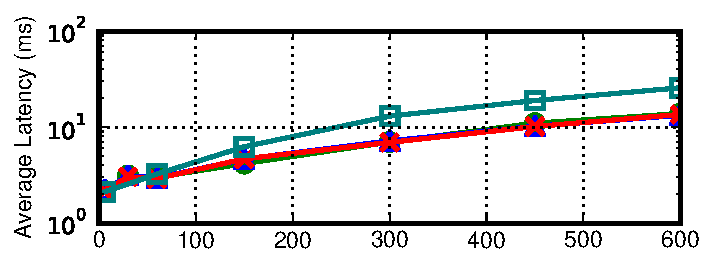
\includegraphics[width=0.90\columnwidth]{figs/lan-threads-lats.pdf}\vspace{-1em}
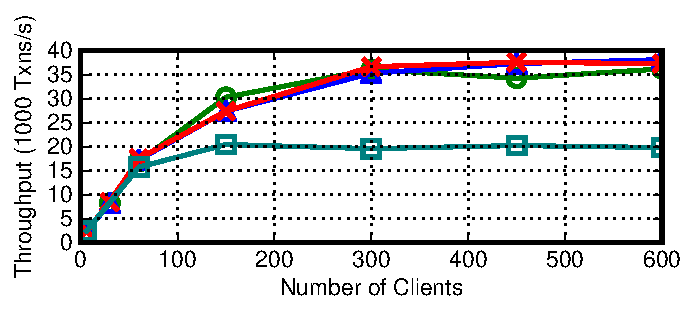
\includegraphics[width=0.90\columnwidth]{figs/lan-threads-thru.pdf}
\begin{center}\textbf{Between \texttt{us-east} and \texttt{us-west-2}}\end{center}\vspace{-1.5em}
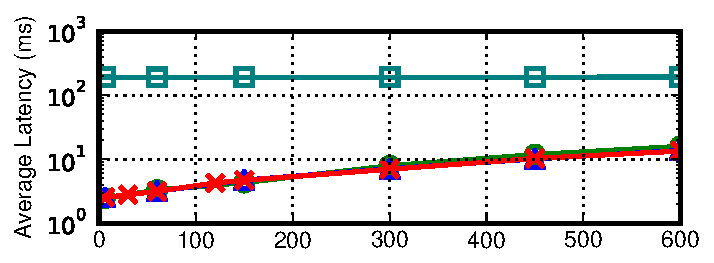
\includegraphics[width=0.90\columnwidth]{figs/wan-threads-lats.pdf}\vspace{-1em}
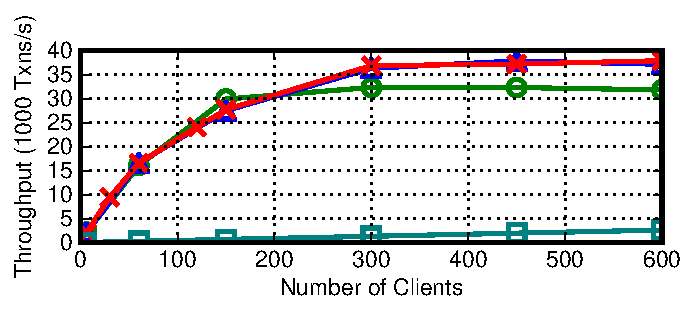
\includegraphics[width=0.90\columnwidth]{figs/wan-threads-thru.pdf}
\caption{YCSB performance for two clusters of three servers each
  deployed within a single datacenter and cross-datacenters.}
\label{fig:wan-exp}
\end{figure}

As Figure~\ref{fig:wan-exp} shows, within a single datacenter, a
mastered implementation achieves approximately double the latency and
slightly over half of the throughput of a HAT implementation. This is
because, given two replicas for each key, the mastered implementation
serves requests from only one. The mastered implementation still
achieves $19,797$ transactions per second---over 6,000 per
master---and is only $15.56$ms slower at peak compared to eventual
consistency. However, eventual consistency and HAT models achieve
substantially higher throughput--$37,575$ and $36,178$ transactions
per second, respectively--and lower latency---$48.3\%$ and $47.2\%$
respectively. This difference is unsurprising because, in these weaker
models, all servers can serve both reads and writes, effectively
doubling the capacity of the system. The weaker models still propagate
new values between replicas, but this process is asynchronous and,
aside from consuming disk I/O and network bandwidth, does not
substantially impact clients. As expected, HAT models perform
similarly to eventual consistency: our Read Committed implementation
buffers client writes and adds no additional server-side overhead,
while TA requires additional metadata with each write but has less
than 5\% performance impact compared to eventual consistency.

In comparison, over multiple datacenters, the cost of coordination
increases. The HAT and eventual consistency implementations continue
to enjoy local RTTs only, and, with the exception of a slight
performance degradation in TA---which we believe is attributable to
Java garbage collection overheads in TA's inbound anti-entropy
buffers---performance remains unchanged. However, each YCSB update to
a remote replica ($\frac{2}{3}$ in one datacenter, $\frac{1}{3}$ in
the other) of requiring a remote RTT between Virginia and Oregon (or
vice-versa) to reach the master. This leads to a latency increase of
around $166$ms ($746\%$) per transaction compared to a
single-datacenter deployment. In order to attain reasonable throughput
for the mastered deployment, we had to greatly increase the number of
concurrent clients accessing the database, and we found that threading
and socket overheads quickly overwhelmed the database server. Over a
wide-area network, the increased cost of RTTs dramatically affects
system efficiency.

This brief set of experiments is not meant as an exhaustive study, but
it validates our earlier intuition about the cost of violating
HAT-compliance. As Deutsch points out, ignoring factors such as
latency can ``cause big trouble and painful learning
experiences''~\cite{fallacies-deutsch}---in a single-site context,
paying the cost of coordination may be tenable, but, especially as
services are geo-replicated,  costs increase. 
